\documentclass[10pt,a4paper]{article}
\usepackage[margin=18mm,top=20mm,bottom=18mm]{geometry}
\usepackage{amsmath,amssymb}
\usepackage{graphicx}
\usepackage{booktabs}
\usepackage{xcolor}
\usepackage[most]{tcolorbox}
\usepackage{titlesec}
\usepackage{caption}
\usepackage{float}
\usepackage{fancyhdr}
\usepackage{enumitem}
\usepackage{siunitx}
\usepackage[colorlinks=true,linkcolor=black,citecolor=black,urlcolor=black]{hyperref}

\definecolor{mid}{HTML}{6E6E6E}
\setlength{\parskip}{2.5pt}
\setlength{\parindent}{0pt}
\captionsetup{font=small,labelfont=bf,skip=3pt}
\titleformat{\section}{\normalsize\bfseries\scshape}{\thesection}{0.6em}{}
\titleformat{\subsection}{\small\bfseries}{\thesubsection}{0.5em}{}
\titlespacing*{\section}{0pt}{6pt}{2pt}
\titlespacing*{\subsection}{0pt}{4pt}{1pt}
\setlist{itemsep=0.5pt,topsep=1.5pt,leftmargin=13pt}
\newcommand{\dfus}{\Delta_{\mathrm{fus}}}
\newcommand{\aoh}{a_{\mathrm{OH}}}
\sisetup{detect-all}

\pagestyle{fancy}\fancyhf{}
\fancyhead[L]{\footnotesize\color{mid}CL207 Chemical Engineering Thermodynamics --- optional project (draft for Checkpoint 3)}
\fancyhead[R]{\footnotesize\color{mid}Chowdhary, 25B0347}
\fancyfoot[C]{\footnotesize\thepage\ / 5}
\renewcommand{\headrulewidth}{0.3pt}

\begin{document}

%===================================================================== PAGE 1
\begin{center}
{\Large\bfseries One constant per hydroxyl group: predicting freeze concentration\\[2pt]
and designing glycerol-sparing cryoprotectant mixtures}\\[7pt]
{\normalsize Siddhant Chowdhary}\\[1pt]
{\small Roll no.\ 25B0347 \quad $\cdot$ \quad Department of Chemical Engineering, IIT Bombay}\\[1pt]
{\small\color{mid}Theme: Thermodynamics in Biological Systems}
\end{center}
\vspace{1pt}

\begin{tcolorbox}[colback=white,colframe=black,boxrule=0.5pt,arc=1pt,left=7pt,right=7pt,top=4pt,bottom=4pt,
  title=Abstract,fonttitle=\bfseries\small,colbacktitle=black,coltitle=white]
\small
Slow freezing concentrates salt in the liquid around cells. Glycerol limits this but is toxic, so its dose
should be no larger than the salt limit requires. Because ice is pure water, solid--liquid equilibrium fixes
the water activity of the unfrozen liquid at each temperature; a recipe changes only how much liquid remains
and how salty it is. We describe water activity with a one-constant excess Gibbs energy model in which the
water--solute interaction is counted per hydroxyl group. The constant was fitted on glycerol freezing points
(RMSE 0.017\,K), fixed in version control, and tested without refitting against independent literature data:
11 solutes, sorbitol and sucrose at 25\,\textdegree C, and the glycerol--NaCl--water phase diagram. It predicted
ethylene glycol and sucrose 3$\times$ and 17$\times$ more accurately than an ideal solution, beat UNIFAC for every
solute except sorbitol, and for glycerol\,+\,NaCl above 30\,wt\% solute was about 3--5$\times$ more accurate than
the two standard cryobiology models. It fails for sorbitol and monohydric alcohols; a two-temperature test
traces the sorbitol failure to the molecule, not to temperature. For design, each gram of sorbitol replaces
0.7--0.9\,g of glycerol at a fixed salt limit, across three activity models and a $\pm25\%$ change in the limit.
\end{tcolorbox}

{\small\textbf{Keywords:} cryopreservation; solid--liquid equilibrium; activity coefficients; group
contribution; freeze concentration; blind prediction}

\vspace{2pt}
\begin{figure}[H]
\centering
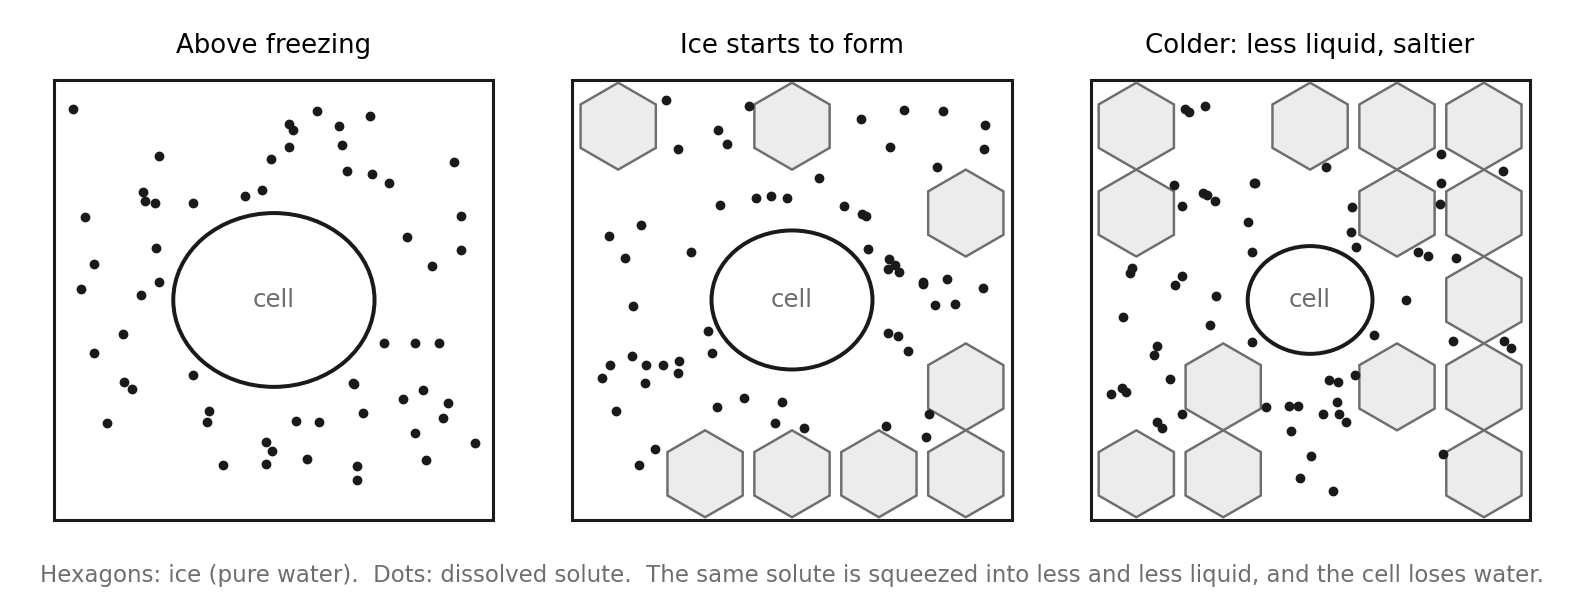
\includegraphics[width=0.93\textwidth]{fig_freeze_concentration.png}
\caption{Freeze concentration. Ice is pure water, so the same salt is squeezed into less and less liquid as
temperature falls, and water leaves the cell. Without a cryoprotectant, our model puts the NaCl content of
the unfrozen liquid of physiological saline (0.9\,wt\%) at 14.0\,wt\% at $-10$\,\textdegree C and 18.8\,wt\% at
$-15$\,\textdegree C; red cells begin to haemolyse at about 4.4\,wt\% \cite{lovelock11,shepard}.}
\label{fig:fc}
\end{figure}

\vspace{-2pt}
{\small\textbf{Status at Checkpoint 3.} All modelling and literature tests are complete and reproducible
from one command (\texttt{python run\_all.py}). Laboratory freezing-point measurements, with predictions
already committed, are scheduled for the coming week.}

\clearpage
%===================================================================== PAGE 2
\section{Introduction and background}

\textbf{The problem.} Cells, tissues and biologics are stored frozen, but freezing can kill them. In slow
freezing, ice forms outside the cells first; the remaining solution becomes progressively concentrated and
water leaves the cells by osmosis. Exposure to this concentrated solution is one arm of Mazur's two-factor
account of freezing injury \cite{mazur}, and the temperature range in which it acts, roughly $-15$ to
$-60$\,\textdegree C, is the one cells must cross on cooling and on warming \cite{gao}. Lovelock showed that
glycerol protects red cells by diluting the salt that would otherwise accumulate \cite{lovelock10,lovelock11}.
Pegg summarises the trade-off: ``Cryoprotectants, simply by increasing the total concentration of all
solutes in the system, reduce the amount of ice formed at any given temperature; but to be biologically
acceptable they must be able to penetrate into the cells and have low toxicity'' \cite{pegg}. The first half
is thermodynamics; the second is why the dose matters, and why non-penetrating sorbitol can share
glycerol's job but not replace it.

\textbf{Alignment with the theme.} The unfrozen liquid's composition is set by ice--solution phase equilibrium,
not by the cell, so choosing a cryoprotectant dose is first a solid--liquid equilibrium (SLE) problem.

\textbf{Relevant principles.} At equilibrium the fugacity of water is the same in ice and in the liquid.
Ice is pure, and building the solid--liquid fugacity ratio along a heat--melt--cool path \cite{sandler} gives
\begin{equation}
\ln(x_w\gamma_w) \;=\; -\frac{\dfus H}{R}\left(\frac{1}{T}-\frac{1}{T_m}\right)
 \;-\; \frac{\Delta C_p}{R}\left(\frac{T_m}{T}-1+\ln\frac{T}{T_m}\right),
\label{eq:sle}
\end{equation}
with $\dfus H=\SI{6009.5}{J\,mol^{-1}}$, $\Delta C_p=\SI{37.9}{J\,mol^{-1}K^{-1}}$ and $T_m=273.15$\,K for water.
The right-hand side depends on $T$ only. \emph{Once ice is present, the water activity of the unfrozen liquid
is fixed by temperature, whatever is dissolved in it.} A cryoprotectant cannot change that activity; it changes
how much water must freeze out before the liquid reaches it, and so how concentrated the salt becomes.
Everything therefore hinges on the activity coefficient $\gamma_w$. For water--polyol mixtures $\gamma_w<1$:
hydroxyl groups hydrogen-bond to water, so a polyol lowers the freezing point more than Raoult's law predicts.

\textbf{Existing approaches.} (i) Many cryobiological models assume ideal, dilute solutions. (ii) The
cryobiology field's non-ideal models are the osmotic virial equation \cite{elliott,zielinski} and the
Kleinhans--Mazur freezing-point summation \cite{km}; both need coefficients fitted separately for every
solute. (iii) A one- and two-parameter Margules model has been fitted to water--glycerol SLE
\cite{zargarzadeh}, so a Margules fit for glycerol alone is not new. (iv) Group-contribution methods
(UNIFAC \cite{unifac}, modified UNIFAC (Dortmund) \cite{dortmund}) predict activity coefficients of any
molecule from group parameters fitted mostly to vapour--liquid data at and above room temperature; polyol-specific
UNIFAC versions have been fitted to water activity at 25\,\textdegree C \cite{marcolli,peres}. A recent review suggests such
models could screen cryoprotectant mixtures but does not apply them to freezing \cite{powellpalm}.

\textbf{Gap and hypothesis.} Per-solute coefficients cannot be used for a molecule that has not been
measured, and general group-contribution parameters are not tuned to freezing. We test a narrow middle
route. \emph{Hypothesis: one water--OH interaction constant, fitted on glycerol only, predicts freezing of
other polyols and of polyol\,+\,salt mixtures without refitting.} Every test was fixed before the test data
were examined, so a negative result is informative rather than a failure of the project: where the
hypothesis breaks tells us which physical assumption broke. The design question then follows directly: how
much glycerol can a non-penetrating polyol replace while the salt in the unfrozen liquid stays below the
damage threshold? This combination --- a transferable per-group constant, blind tests against cryobiology's
own models, and a glycerol-sparing design --- was not found in this form in the literature we searched.

\clearpage
%===================================================================== PAGE 3
\section{Methodology}

\begin{figure}[H]
\centering
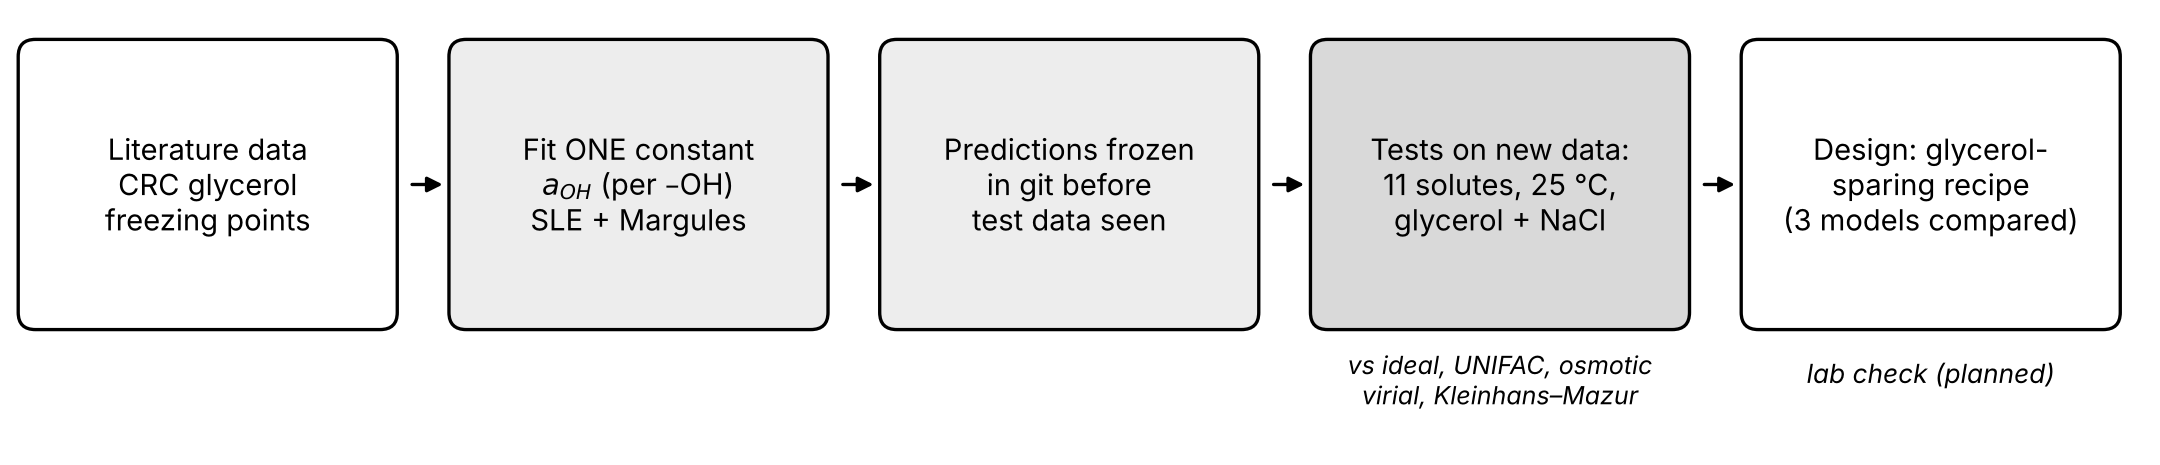
\includegraphics[width=\textwidth]{report_pipeline.png}
\caption{Workflow. One constant is fitted on glycerol, frozen in version control, and then tested against
data it has never seen before being used for design.}
\label{fig:pipeline}
\end{figure}
\vspace{-6pt}

\subsection{Activity model with one constant per hydroxyl group}
Only water--solute pair interactions are kept (one-constant Margules for each solute), and the interaction
of solute $i$ is assumed proportional to its number of hydroxyl groups:
\begin{equation}
\frac{G^{\mathrm{ex}}}{RT} = x_w\sum_i \alpha_i x_i,\qquad
\alpha_i = \frac{n_{\mathrm{OH},i}\,\aoh}{RT},\qquad
\ln\gamma_w = (1-x_w)\sum_i \alpha_i x_i .
\label{eq:model}
\end{equation}
Glycerol has 3 OH, ethylene glycol and propylene glycol 2, sorbitol and mannitol 6, sucrose 8. The single
constant $\aoh$ is fitted by least squares to 19 CRC freezing points of glycerol, 2--40\,wt\% \cite{crc}, by
solving (\ref{eq:sle})--(\ref{eq:model}) for $T$. The interaction energy is assumed independent of
temperature, so $\alpha_i$ scales as $1/T$; this assumption was written down before any test at another
temperature.

\subsection{Salt and the mixing rule}
NaCl is strongly non-ideal (Debye--H\"uckel behaviour), so it is described by an empirical osmotic
coefficient fitted to the CRC NaCl ice line \cite{crc}: $\ln a_w^{\mathrm{NaCl}} = -2mM_w\phi(m)$,
$\phi = 1 - a\sqrt m/(1+\sqrt m) + bm + cm^2$ ($m$ in mol\,kg$^{-1}$; RMSE 0.023\,K to the eutectic).
For mixtures we add contributions to $\ln a_w$ at the mixture's molalities, with no salt--polyol cross term.
This rule follows from the activity framework; it was chosen before any mixture data were seen, and the
cryobiology alternative (adding freezing-point depressions \cite{km}) is reported as a comparison only.

\subsection{Blind tests and benchmarks}
After the fit, predictions were committed to a git repository and never edited; new data were then entered
and compared. The test data are all independent of the fit:
\begin{itemize}
\item \textbf{Single solutes, near 0\,\textdegree C:} CRC freezing points for ethylene glycol, mannitol,
methanol, ethanol, 1- and 2-propanol, glucose, fructose and sucrose \cite{crc}; sorbitol from a cryoscope study
(1--11\,wt\%) \cite{baer} and DSC (35--64\,wt\%) \cite{siniti}; propylene glycol via a published correlation \cite{zielinski}.
\item \textbf{Another temperature:} isopiestic osmotic coefficients of sorbitol \cite{bower} and sucrose
\cite{robinson} at 25\,\textdegree C.
\item \textbf{Salt mixtures:} the water--glycerol--NaCl liquidus of Shepard et al.\ \cite{shepard}. The paper
gives no tables, so its Fig.~3 (nine glycerol:NaCl ratios) was digitised by hand (76 points; calibration
checked against the NaCl--water eutectic). Pass criterion, fixed in advance: RMS error $\le 0.5$\,K for total
solute $\le 30$\,wt\%. The sorbitol\,+\,NaCl data of \cite{bower} test the neglected cross term.
\end{itemize}
Every test is run against the ideal solution, UNIFAC and Dortmund UNIFAC \cite{unifac,dortmund,thermo}, and, for
mixtures, the osmotic virial equation and the Kleinhans--Mazur summation with published coefficients
\cite{zielinski,km}.

\subsection{Recipe design}
For 0.9\,wt\% saline with a sorbitol dose $w_s$, we find the smallest glycerol dose $w_g$ that keeps NaCl in
the unfrozen liquid at or below 4.41\,wt\%, the onset of red-cell haemolysis \cite{lovelock11,shepard}, at
$-15$\,\textdegree C, the top of the lethal range \cite{gao} (also $-10$ and $-20$\,\textdegree C). The unfrozen
fraction comes from a water balance solved with (\ref{eq:sle}). No toxicity weights are used, because none could
be sourced for sorbitol. The design is repeated with the ideal and UNIFAC models to see whether the
conclusion depends on the activity model.

\subsection{Planned measurements}
Freezing points by cooling curve (calibrated DS18B20 probes, ice--salt bath, maximum after recalescence):
glycerol 30\,wt\% as a method check against CRC; propylene glycol 30, sorbitol 40, glycerol 15\,+\,sorbitol 15 and
glycerol 20\,+\,NaCl 5\,wt\%, in duplicate. The models' predictions for these samples differ by 0.7--6.6\,K,
far more than the expected measurement error ($\approx$0.3\,K), so each measurement discriminates.

\clearpage
%===================================================================== PAGE 4
\section{Preliminary results and discussion}

\begin{figure}[H]
\centering
\includegraphics[width=0.96\textwidth]{report_results.png}
\caption{(a) Freezing-point error of each model on single solutes it was not fitted to (log scale). Right of
the dotted line: concentrated sorbitol, where the hypothesis fails. (b) Error on the glycerol\,+\,NaCl\,+\,water
liquidus \cite{shepard}; all three models predict from single-solute data only. (c) Minimum glycerol that keeps
NaCl in the unfrozen liquid $\le 4.41$\,wt\% at $-15$\,\textdegree C, against sorbitol added.}
\label{fig:results}
\end{figure}
\vspace{-6pt}

\begin{table}[H]
\centering\footnotesize\setlength{\tabcolsep}{4pt}
\caption{Summary of tests. Error = model minus data. $a_{\mathrm{OH}} = -2414.9$\,J\,mol$^{-1}$ per OH, never refitted.}
\label{tab:results}
\begin{tabular}{@{}llccccl@{}}
\toprule
Test & Metric & Per-OH & Ideal & UNIFAC & Other & Verdict \\
\midrule
Glycerol, 2--40\,wt\% (fit) & RMSE, K & 0.02 & 1.31 & 2.1 & 0.27$^a$ & fit only \\
Ethylene glycol, 2--40\,wt\% & RMSE, K & \textbf{0.83} & 2.49 & 3.99 & 0.52$^a$ & transfers \\
Sucrose / glucose, to 40\,wt\% & RMSE, K & \textbf{0.02} / 0.12 & 0.35 / 0.23 & -- & 0.02 / 0.01$^a$ & transfers \\
Methanol / ethanol & RMSE, K & 2.20 / 2.57 & 4.84 / 4.12 & 7.17 / 9.13 & 1.29 / 0.91$^a$ & fails \\
Sorbitol, 53--64\,wt\% & RMSE, K & 4.7 & 5.3 & \textbf{1.6} & -- & fails \\
Sorbitol, 25\,\textdegree C, 0.9--3.7\,mol\,kg$^{-1}$ & RMS in $\phi$ & 0.163 & \textbf{0.060} & 0.113 & -- & fails \\
Glycerol\,+\,NaCl, $\le$30\,wt\% solute & RMS, K & 0.69 & 0.89$^b$ & -- & 0.69$^a$ / 0.59$^c$ & misses 0.5\,K \\
Glycerol\,+\,NaCl, $>$30\,wt\% solute & RMS, K & \textbf{1.23} & 4.64$^b$ & -- & 5.75$^a$ / 3.39$^c$ & best \\
\bottomrule
\end{tabular}\\[1pt]
{\footnotesize $^a$osmotic virial, coefficients fitted per solute \cite{zielinski} (in-sample for single solutes);
$^b$ideal glycerol\,+\,fitted NaCl; $^c$Kleinhans--Mazur summation.}
\end{table}
\vspace{-4pt}

\textbf{Where the hypothesis holds.} For ethylene glycol, glycerol and sucrose --- polyols with about one
hydroxyl per carbon --- a constant fitted on glycerol predicts freezing without refitting, and as well as
osmotic virial coefficients fitted to each molecule separately (Table~\ref{tab:results}). For the
glycerol\,+\,NaCl liquidus it missed the pre-set 0.5\,K target at low concentration (0.69\,K). The figure itself
is uncertain by about 0.34\,K (its pure-glycerol and pure-NaCl edges against CRC data), and all three
mixture models agree within 0.1\,K there. Above 30\,wt\% solute --- the conditions cells actually meet during
freezing --- the additive-$\ln a_w$ rule is about 3$\times$ more accurate than the cryobiology models
(Fig.~\ref{fig:results}b). Sorbitol--NaCl data \cite{bower} show the neglected cross term (salting-in) costs
only 0.05--0.13\,K at the recipe's conditions.

\textbf{Where it fails, and why.} The model overstates the non-ideality of sorbitol: by 3.5--5.5\,K for
concentrated solutions and four- to five-fold in $\phi-1$ at 25\,\textdegree C. Is the cause temperature or the molecule? Sucrose answers this. On the freezing line it implies $\aoh \approx -2200$\,J\,mol$^{-1}$
(close to glycerol's $-2415$), and at 25\,\textdegree C about $-1800$: a real but modest temperature effect.
Sorbitol at the same 25\,\textdegree C implies only $-400$ to $-750$. The failure is therefore mainly the
molecule. A plausible cause, consistent with the proximity correction used for sugars \cite{peres}, is that adjacent hydroxyls on a flexible C$_6$ chain bond to each other rather
than to water, so counting them independently overstates their pull on water. Monohydric alcohols also fail;
their back-calculated constants scatter with no trend in chain length, so a simple CH$_x$ correction is not
supported. One sorbitol dataset \cite{baer} is flagged: it implies $\phi\approx1.14$ at 1\,wt\%, where $\phi$ must approach 1.

\textbf{Ours versus UNIFAC.} UNIFAC is general: many group parameters, fitted mostly to vapour--liquid data
at and above room temperature, none to this system. For water--glycerol it predicts $\gamma_w>1$, the wrong
sign, and under-predicts the depression by up to $\sim$6\,K at 40\,wt\%. Our model is narrow: one group, one
constant, fitted on freezing data. It gets the sign and size right for the polyols it covers and fails outside
them, where UNIFAC is sometimes better (concentrated sorbitol). The trade-off is breadth against accuracy
in one class of molecules.

\textbf{Design result and practicability.} At $-15$\,\textdegree C without sorbitol, the minimum glycerol is
6.5 (per-OH), 7.6 (ideal) or 8.4\,wt\% (UNIFAC). The dose depends on the model and on the salt limit
(4.9--9.2\,wt\% for a $\pm25\%$ change). The \emph{replacement ratio} does not: each gram of sorbitol saves
0.68--0.91\,g of glycerol across all 27 combinations of model, temperature and salt limit
(Fig.~\ref{fig:results}c). The zero-glycerol end is thermodynamically allowed but biologically unacceptable,
because sorbitol does not enter cells \cite{pegg}. Measuring the recipe's freezing point barely tests it (the models differ by 0.14\,K); measuring the salt in the
unfrozen liquid would.

\clearpage
%===================================================================== PAGE 5
\section{Conclusion and next steps}

\textbf{Conclusion.} A single hydroxyl-group constant, fitted on one molecule, predicts freezing of small
polyols and sucrose, and of glycerol\,+\,salt mixtures, without refitting. It matches per-molecule cryobiology
models at low concentration and beats them where solutions are concentrated. It fails for sorbitol and for
monohydric alcohols, and the tests locate why. For cryoprotectant design, the useful output is not a
single recipe but a robust exchange rate: about 0.7--0.9\,g of glycerol saved per gram of sorbitol, whichever
activity model is used.

\textbf{Potential impact.} Survival assays take days each; a model calibrated on one molecule covers the
composition axis continuously, so experiments can be kept for confirmation.

\textbf{Scope.} The model predicts the liquid a cell sits in, not survival; toxicity, transport and intracellular ice are outside it.

\textbf{Next steps.}
\begin{enumerate}
\item \textbf{Laboratory check (next week).} Measure the five committed samples (Section~2.5) and compare
with all models without refitting; glycerol 30\,wt\% calibrates the method.
\item \textbf{Post-hoc analysis, labelled as such:} one constant per molecule, to test whether hydroxyl spacing explains the spread.
\item \textbf{Cross-check UNIFAC} numbers in an independent simulator (DWSIM or Aspen Plus).
\item \textbf{If time allows:} equilibrium cell volume during freezing (Boyle--van't Hoff), from the same water activity.
\end{enumerate}

\textbf{Code and data.} All code, data and committed predictions are in a git repository (link to be added);
\texttt{python run\_all.py} rebuilds every figure and table and checks the predictions reproduce.

\renewcommand{\refname}{\normalsize\bfseries\scshape References}
\begin{thebibliography}{99}
\footnotesize
\setlength{\itemsep}{0pt}\setlength{\parsep}{0pt}
\bibitem{mazur} P. Mazur, Freezing of living cells: mechanisms and implications, \emph{Am.\ J.\ Physiol.} 247 (1984) C125--C142. doi:10.1152/ajpcell.1984.247.3.C125
\bibitem{gao} D. Gao, J.\,K. Critser, Mechanisms of cryoinjury in living cells, \emph{ILAR J.} 41 (2000) 187--196. doi:10.1093/ilar.41.4.187
\bibitem{lovelock10} J.\,E. Lovelock, The haemolysis of human red blood-cells by freezing and thawing, \emph{Biochim.\ Biophys.\ Acta} 10 (1953) 414--426. doi:10.1016/0006-3002(53)90273-x
\bibitem{lovelock11} J.\,E. Lovelock, The mechanism of the protective action of glycerol against haemolysis by freezing and thawing, \emph{Biochim.\ Biophys.\ Acta} 11 (1953) 28--36. doi:10.1016/0006-3002(53)90005-5
\bibitem{pegg} D.\,E. Pegg, Principles of cryopreservation, \emph{Methods Mol.\ Biol.} 368 (2007) 39--57. doi:10.1007/978-1-59745-362-2\_3
\bibitem{sandler} S.\,I. Sandler, \emph{Chemical, Biochemical, and Engineering Thermodynamics}, 4th ed., Wiley, 2006.
\bibitem{elliott} J.\,A.\,W. Elliott et al., A multisolute osmotic virial equation for solutions of interest in biology, \emph{J.\ Phys.\ Chem.\ B} 111 (2007) 1775--1785. doi:10.1021/jp0680342
\bibitem{zielinski} M.\,W. Zielinski et al., Comparison of non-ideal solution theories for multi-solute solutions in cryobiology and tabulation of required coefficients, \emph{Cryobiology} 69 (2014) 305--317. doi:10.1016/j.cryobiol.2014.08.005
\bibitem{km} F.\,W. Kleinhans, P. Mazur, Comparison of actual vs.\ synthesized ternary phase diagrams for solutes of cryobiological interest, \emph{Cryobiology} 54 (2007) 212--222. doi:10.1016/j.cryobiol.2007.01.007
\bibitem{zargarzadeh} L. Zargarzadeh, J.\,A.\,W. Elliott, Comparison of the osmotic virial equation with the Margules activity model for solid--liquid equilibrium, \emph{J.\ Phys.\ Chem.\ B} 123 (2019) 1099--1107. doi:10.1021/acs.jpcb.8b09285
\bibitem{unifac} Aa. Fredenslund, R.\,L. Jones, J.\,M. Prausnitz, Group-contribution estimation of activity coefficients in nonideal liquid mixtures, \emph{AIChE J.} 21 (1975) 1086--1099.
\bibitem{dortmund} U. Weidlich, J. Gmehling, A modified UNIFAC model. 1. Prediction of VLE, $h^E$, and $\gamma^\infty$, \emph{Ind.\ Eng.\ Chem.\ Res.} 26 (1987) 1372--1381.
\bibitem{marcolli} C. Marcolli, Th. Peter, Water activity in polyol/water systems: new UNIFAC parameterization, \emph{Atmos.\ Chem.\ Phys.} 5 (2005) 1545--1555. doi:10.5194/acp-5-1545-2005
\bibitem{peres} A.\,M. Peres, E.\,A. Macedo, A modified UNIFAC model for the calculation of thermodynamic properties of aqueous and non-aqueous solutions containing sugars, \emph{Fluid Phase Equilib.} 139 (1997) 47--74. doi:10.1016/S0378-3812(97)00196-9
\bibitem{powellpalm} M.\,J. Powell-Palm, A.\,N. Consiglio, Thermodynamic principles of emerging cryopreservation technologies, arXiv:2601.12573 (2026).
\bibitem{thermo} C. Bell et al., \emph{thermo} (Python package), v0.6.1, \url{https://github.com/CalebBell/thermo}.
\bibitem{crc} D.\,R. Lide (ed.), \emph{CRC Handbook of Chemistry and Physics}, Internet Version 2005, pp.\ 8-58 to 8-84.
\bibitem{baer} R.\,J. Baer, K.\,A. Baldwin, Freezing points of bulking agents used in manufacture of low-calorie frozen desserts, \emph{J.\ Dairy Sci.} 67 (1984) 2860--2862.
\bibitem{siniti} M. Siniti, S. Jabrane, J.\,M. L\'etoff\'e, Study of the respective binary phase diagrams of sorbitol with mannitol, maltitol and water, \emph{Thermochim.\ Acta} 325 (1999) 171--180.
\bibitem{bower} V.\,E. Bower, R.\,A. Robinson, Isopiestic vapor pressure measurements of the ternary system: sorbitol--sodium chloride--water at 25\textdegree, \emph{J.\ Phys.\ Chem.} 67 (1963) 1540--1541. doi:10.1021/j100801a033
\bibitem{robinson} R.\,A. Robinson, R.\,H. Stokes, Tables of osmotic and activity coefficients of electrolytes in aqueous solution at 25\,\textdegree C, \emph{Trans.\ Faraday Soc.} 45 (1949) 612--624.
\bibitem{shepard} M.\,L. Shepard, C.\,S. Goldston, F.\,H. Cocks, The H$_2$O--NaCl--glycerol phase diagram and its application in cryobiology, \emph{Cryobiology} 13 (1976) 9--23. doi:10.1016/0011-2240(76)90154-1
\end{thebibliography}

\end{document}
